
        \documentclass{article}
        \usepackage[utf8]{inputenc}
        \usepackage[spanish]{babel}
        \usepackage{amsmath}
        \usepackage{graphicx}
        \usepackage{float}
        \usepackage{setspace}
        \usepackage{siunitx}
        \usepackage{geometry}
        \geometry{
            left=1in,
            right=1in,
            top=1in,
            bottom=1in
        }
        \doublespacing
        \begin{document}
        \section{Modelo de la catapulta}
        \begin{figure}[H]
            \centering
            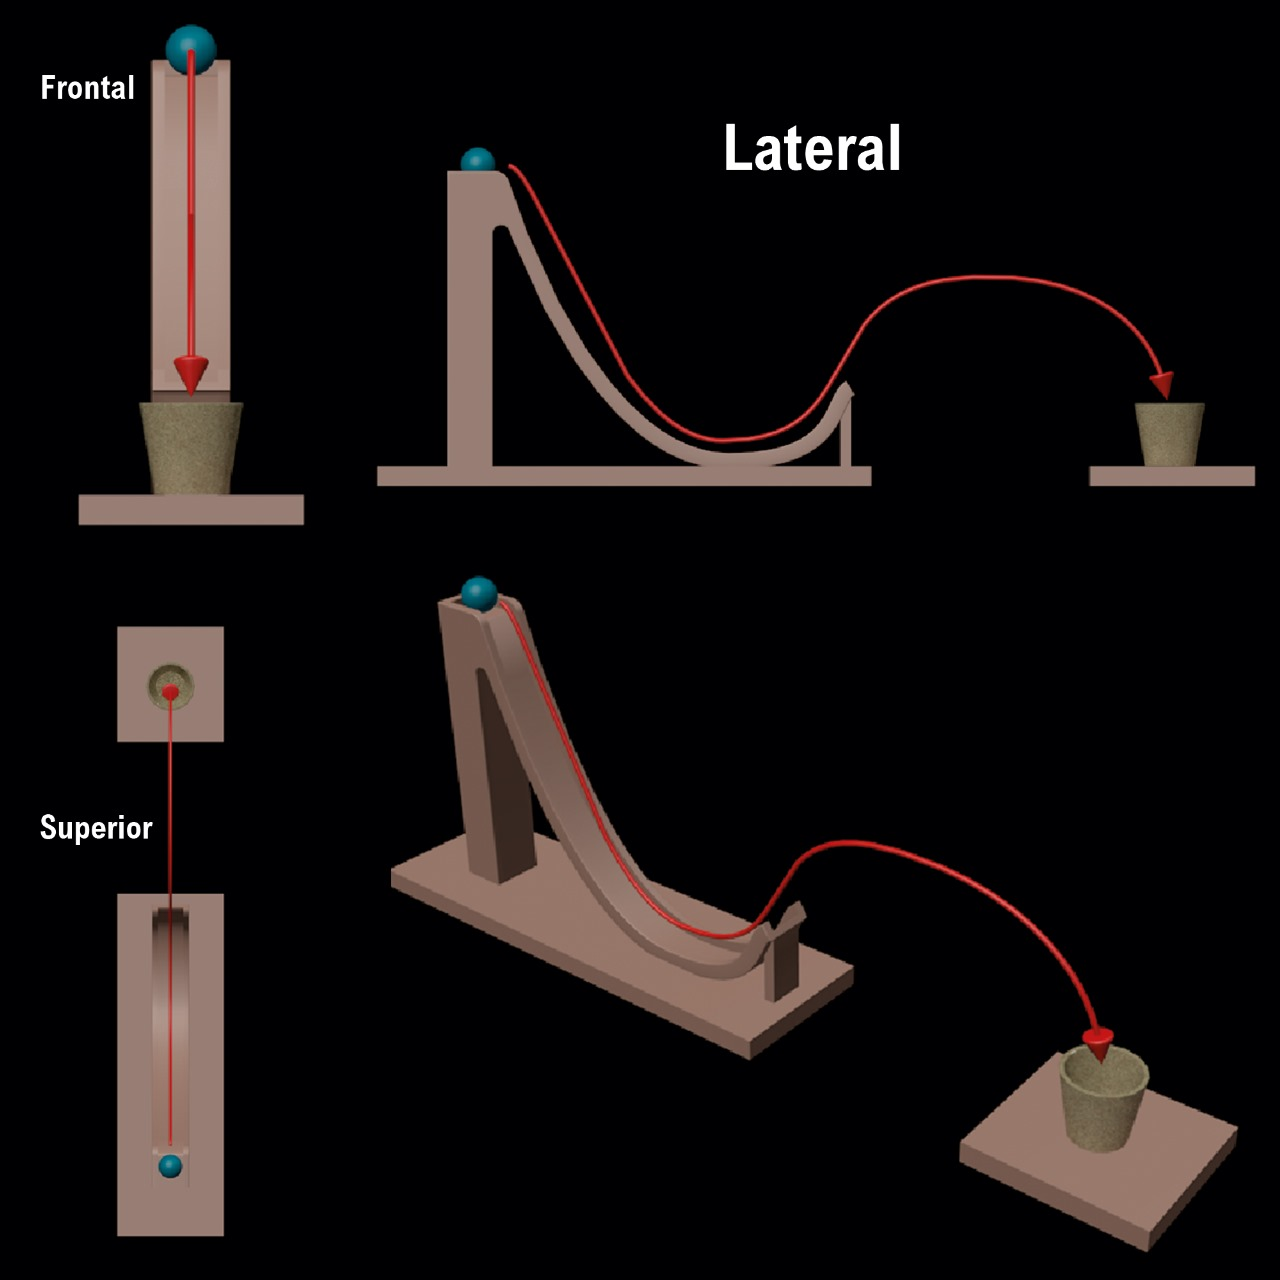
\includegraphics[width=0.5\textwidth]{figures/catapulta.jpeg}
            \caption{Modelo de la catapulta}
        \end{figure}
        \section{Variables}
        Las variables iniciales son:
        \begin{align*}
            m &= 0.1 \si{kg} \\
            g &= 9.81 \si{m/s^2} \\
            h_A &= 0.5 \si{m} \\
            h_B &= 0.05 \si{m} \\
            \theta_B &= 25 \si{\degree} \\
        \end{align*}
        
        \section{Cálculos (sin fricción)}
        En este caso, se asume que no hay fricción entre el proyectil y la rampa ni entre el proyectil y el aire, por lo que la energía mecánica se conserva a lo largo de todo el trayecto, desde que se suelta el proyectil en el punto $A$ hasta que cae al suelo.
        \subsection{Velocidad en el punto $B$}
        Para calcular la velocidad con la que el proyectil sale disparado de la rampa, o la velocidad en el punto $B$,
        se utiliza la conservación de la energía mecánica.
        \begin{align*}
            E &= K + U \\
        \end{align*}
        Donde:
        \begin{align*}
            K &= \frac{1}{2} m v^2 \\
            U &= m g h \\
        \end{align*}
        Como no hay fricción, la energía mecánica se conserva, y la energía en los puntos $A$ y $B$ es la misma:
        \begin{align*}
            E_A &= E_B \\
            K_A + U_A &= K_B + U_B \\
            \frac{1}{2} m v_A^2 + m g h_A &= \frac{1}{2} m v_B^2 + m g h_B \\
        \end{align*}
        Dado que en el punto $A$, el proyectil parte del reposo, $v_A = 0$:
        \begin{align*}
            m g h_A &= \frac{1}{2} m v_B^2 + m g h_B \\
        \end{align*}
        Despejando $v_B$:
        \begin{align*}
            v_B &= \sqrt{v_A^2 + 2 g (h_A - h_B)} \\
        \end{align*}
        Sustituyendo los valores, tenemos:
        \begin{align*}
            v_B &= \sqrt{2 \cdot 9.81 \cdot (0.5 - 0.05)} \\
            v_B &= 2.97 \, \si{m/s} \\
        \end{align*}
        
        \subsection{Funciones de posición}
        Las funciones de posición en función del tiempo de un movimiento parabólico son:
        \begin{align*}
            x(t) &= x_B + v_{xB} t \\
            y(t) &= h_B + v_{yB} t - \frac{1}{2} g t^2 \\
        \end{align*}
        Para descomponer $v_B$ en sus componentes $v_{xB}$ y $v_{yB}$, se tiene:
        \begin{align*}
            v_{xB} &= v_B \cos(\theta_B) \\
            v_{yB} &= v_B \sin(\theta_B) \\
        \end{align*}
        Sustituyendo los valores, tenemos:
        \begin{align*}
            v_{xB} &= 2.97 \cos(25) \\
            v_{yB} &= 2.97 \sin(25) \\
        \end{align*}
        Resolviendo, se tiene:
        \begin{align*}
            v_{xB} &= 2.69 \si{m/s} \\
            v_{yB} &= 1.26 \si{m/s} \\
        \end{align*}
        Sustiyendo las velocidades en las funciones de posición, se obtiene:
        \begin{align*}
            x(t) &= 2.69 t \\
            y(t) &= 0.05 + 1.26 t - \frac{1}{2} 9.81 t^2 \\
        \end{align*}
        Para graficar la trayectoria, parametrizamos las funciones de posición en función del tiempo:
        \[
        \begin{cases}
            x(t) = 2.69 t \\
            y(t) = 0.05 + 1.26 t - \frac{1}{2} 9.81 t^2 \\
        \end{cases}
        \]
        Graficando la ecuación paramétrica, se obtiene:
        \begin{figure}[H]
            \centering
            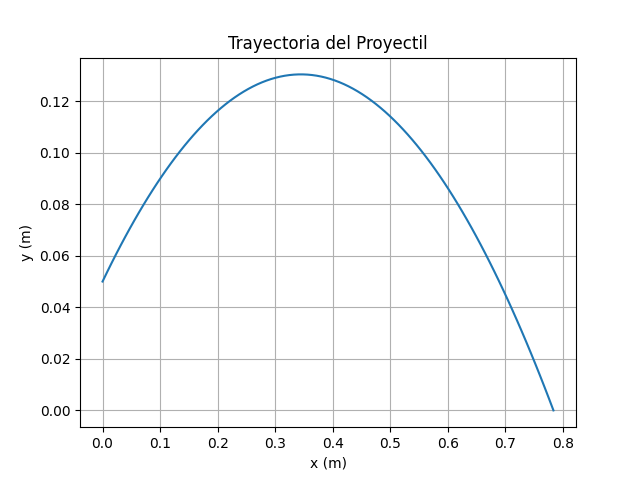
\includegraphics[width=0.8\textwidth]{figures/trayectoria.png}
            \caption{Trayectoria del proyectil}
        \end{figure}
        
        \subsection{Funciones de energía}
        Las funciones de energía en función del tiempo del proyectil son:
        \begin{align*}
            K(t) &= \frac{1}{2} m (v_x(t)^2 + v_y(t)^2) \\
            U(t) &= m g y(t) \\
            E(t) &= K(t) + U(t) \\
        \end{align*}
        Graficando las energías:
        \begin{figure}[H]
            \centering
            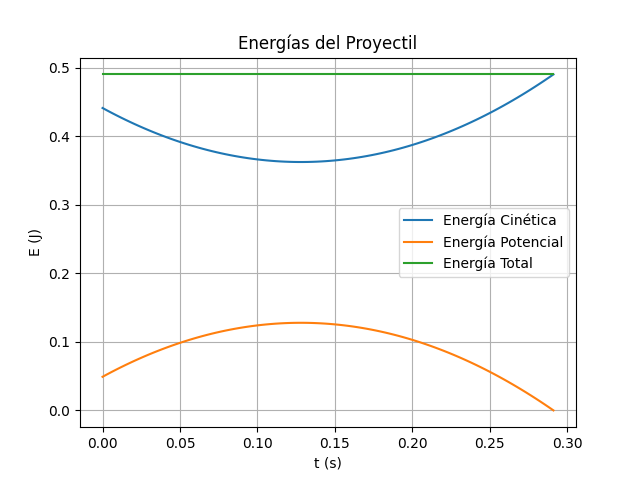
\includegraphics[width=0.8\textwidth]{figures/energia.png}
            \caption{Energías del proyectil}
        \end{figure}
        Como se observa en el gráfico, la energía mecánica se conserva a lo largo de todo el trayecto.
        
        \subsection{Funciones de velocidad}
        Para calcular la velocidad en función del tiempo, derivamos las funciones de posición con respecto al tiempo:
        \begin{align*}
            v_x(t) &= \frac{dx}{dt} = v_{xB} \\
            v_y(t) &= \frac{dy}{dt} = v_{yB} - g t \\
        \end{align*}
        Sustituyendo los valores:
        \begin{align*}
            v_x(t) &= 2.69 \\
            v_y(t) &= 1.26 - 9.81 t \\
        \end{align*}
        Graficando las velocidades:
        \begin{figure}[H]
            \centering
            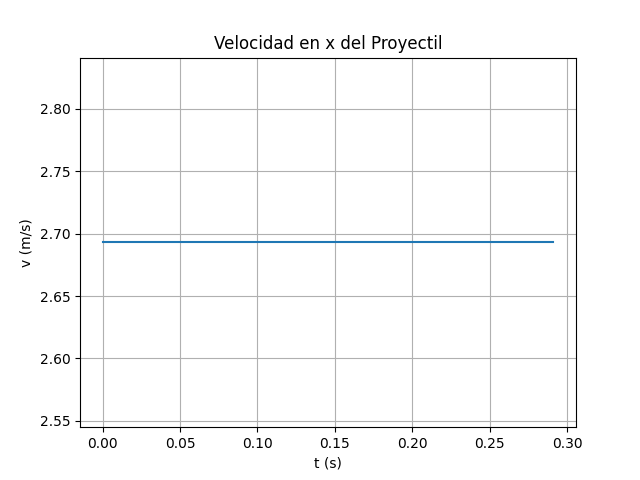
\includegraphics[width=0.8\textwidth]{figures/velocidad_x.png}
            \caption{Velocidad en x del proyectil}
        \end{figure}
        \begin{figure}[H]
            \centering
            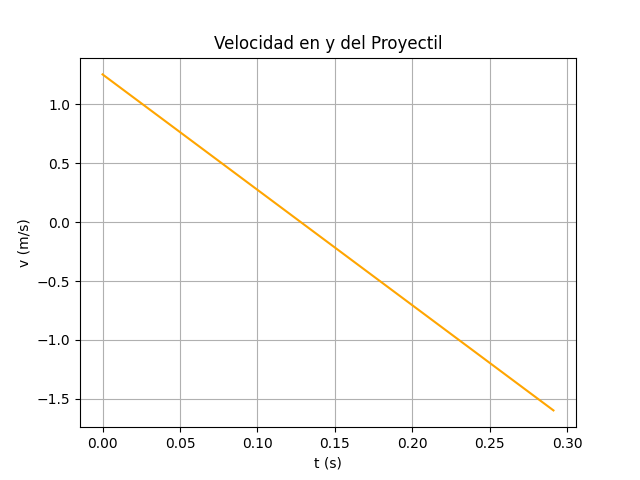
\includegraphics[width=0.8\textwidth]{figures/velocidad_y.png}
            \caption{Velocidad en y del proyectil}
        \end{figure}
        
        \subsection{Tiempo de vuelo}
        El tiempo de vuelo del proyectil es:
        \[
        t = \frac{v_{yB} + \sqrt{v_{yB}^2 + 2 g h_B}}{g}
        \]
        Sustituyendo los valores:
        \begin{align*}
        t &= \frac{ 1.26 + \sqrt{ 1.26^2 + 2 \cdot 9.81 \cdot 0.05 } }{ 9.81 } \\
        t &= 0.29 \, \si{s}
        \end{align*}
        
        \subsection{Alcance}
        El alcance del proyectil es:
        \[
        R = v_{xB} \frac{v_{yB} + \sqrt{v_{yB}^2 + 2gh_B}}{g}
        \]
        Sustituyendo los valores:
        \begin{align*}
        R &= 2.69 \frac{ 1.26 + \sqrt{ 1.26^2 + 2 \cdot 9.81 \cdot 0.05 } }{ 9.81 } \\
        R &= 0.78 \, \si{m}
        \end{align*}
        
        \subsection{Altura máxima}
        La altura máxima alcanzada por el proyectil es:
        \[
        h_{\text{max}} = h_B + \frac{v_B^2 \sin^2(\theta_B)}{2 g}
        \]
        Sustituyendo los valores:
        \begin{align*}
        h_{\text{max}} &= 0.05 + \frac{ 2.97^2 \sin^2(25)}{2 \cdot 9.81} \\
        h_{\text{max}} &= 0.13 \, \si{m}
        \end{align*}
        
        \end{document}
        